%%This is a very basic article template.
%%There is just one section and two subsections.
% \documentclass{article}
%\documentclass[phd,ilcc,twoside]{infthesis}
\documentclass[bsc,logo]{infthesis}
\course{Institute for Language, Cognition and Computation}
\project{\textbf{Supervisor}: Prof. XYZ}

% This package is for times font
\usepackage{times}

% This package is for Informatics thesis style
\usepackage{eushield}

% This package is for your references
\usepackage{natbib}

% This package is for figures
\usepackage{graphicx}

% This package is for urls
\usepackage{url}

% For symbols and equations 
\usepackage{latexsym}
\usepackage{amsmath}

%% Information about the title, etc.
\title{Personalized Air Quality Visualization and Tracking}
\author{Alberto Vazquez Martinez}

%% Specify the abstract here.
\abstract{%

Abstract for my Report
}

\begin{document}

%% First, the preliminary pages
\begin{preliminary}

\maketitle

%% Create the table of contents
\tableofcontents
\listoffigures
\listoftables

\end{preliminary}

\chapter{Introduction}
Here comes the introduction

\chapter{Research Problem}
\label{sec:problem}
Research Problem is to prove that 1 == 2.

\section{How to use section}
\label{sec:probSubSec}
This is an example section.

\subsection{How to use subsection}
This is the subsection.

\chapter{Useful Examples}
\section{How to insert figures?}
Figure \ref{fig:gull} displays a bird. There are different properties for figures. If you want to insert a figure just below this line, just use \texttt{\textbackslash includegraphics} without embedding in the class

\texttt{\textbackslash begin\{figure\}}.

\begin{figure}[h!]
  \centering
    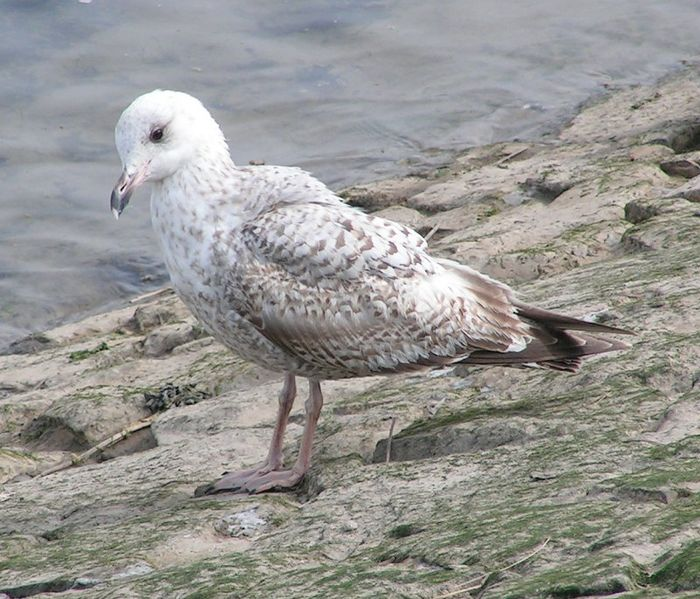
\includegraphics[width=0.5\textwidth]{gull}
    \caption{A picture of a gull.}
    \label{fig:gull3} 
\end{figure} 

More advanced features described at
\url{http://en.wikibooks.org/wiki/LaTeX/Floats,_Figures_and_Captions}

\section{Labeling}
Labels are great way to refer to sections, figures, tables or anything. Here I can refer to Section \ref{sec:probSubSec} since I already defined a label for it using the command \texttt{\textbackslash label}.

\section{How to use references}

We use a phrase structure to ccg conversion algorithm \citep{Hockenmaier:2002} for our experiments.

\cite{Hockenmaier:2002} proposed an algorithm for this purpose. 

See the differences in paranthesis.

You could also use multiple references at the same time just like
\citep{Clark-et-al:2002,ClarkNCurran07}.

You just need to change \texttt{\textbackslash bibliographystyle{xxxxx}} to have
different styles of referencing.

Here is a great document if you would like to try various styles
\url{http://gking.harvard.edu/files/natnotes2.pdf}.

\section{How to use an url?}

Many datasets can be downloaded from \url{http://sivareddy.in/downloads}. 

Documentation of urls at \url{http://en.wikibooks.org/wiki/LaTeX/Hyperlinks}

\section{Table}

\begin{table}[h]
\centering
\begin{tabular}{ l | c || r }
\hline
  1 & 2 & 3 \\
  4 & 5 & 6 \\
\hline
  7 & 8 & 9 \\
\hline
\end{tabular}
\end{table}

Additional documentation on tables at
\url{http://en.wikibooks.org/wiki/LaTeX/Tables}.

\section{Simple Maths}
This is a simple equation $\pi r^2$. Complicated equations can also be written
such as Equation \ref{eqn:main}. You can write any equation. All you need is to
Google for latex symbols or use eclipse suggestion if you have basic idea of symbol names.

 \begin{equation}
 \centering
 \label{eqn:main}
 arg\,max_{L', M} \; \left[ \Bigg(  \prod_{\substack{ w_i \in S \\  (w_i, l_j) 
 \in L'  }} \phi(w_i, l_j, S, B) \Bigg) \psi(M, L', S, B) \right]
 \end{equation}

Documentation on math package and list of symbols is at
\url{http://en.wikibooks.org/wiki/LaTeX/Mathematics}.


All the best with latex and have fun.


\bibliography{references}
\bibliographystyle{apalike}
\end{document}
